\documentclass{standalone}
\usepackage{tikz}
\usetikzlibrary{automata,positioning}

\begin{document}

    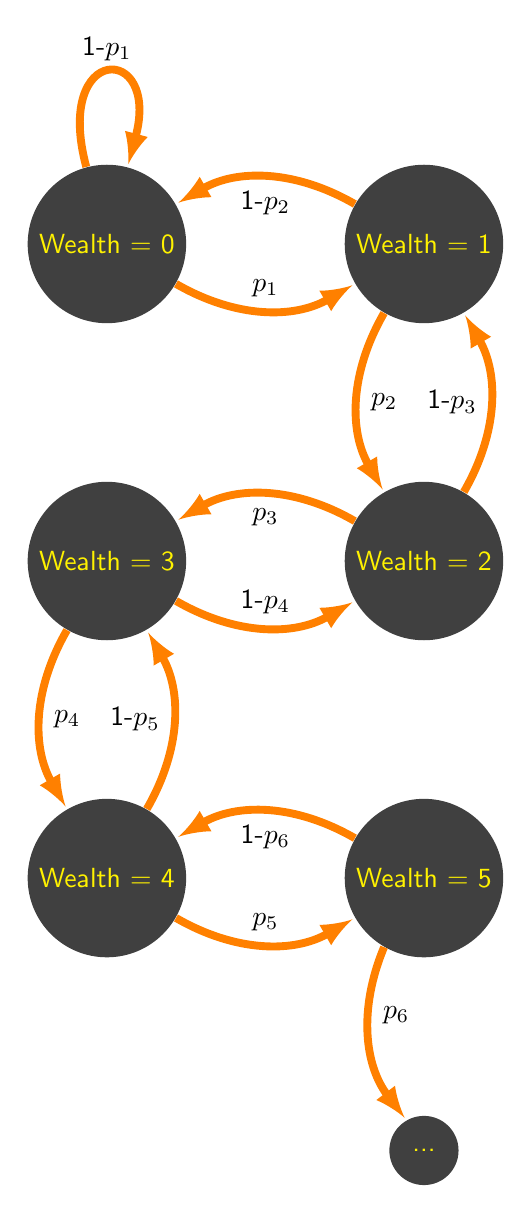
\begin{tikzpicture}[font=\sffamily]
   \node[state,
          text=yellow, 
          draw=none, 
          fill=gray!50!black] (0w) {Wealth = 0};
   \node[state,
          right=2cm of 0w,
          text=yellow, 
          draw=none, 
          fill=gray!50!black] (1w) {Wealth = 1};
    \node[state,
          below=2cm of 1w,
          text=yellow,
          draw=none,
          fill=gray!50!black] (2w) {Wealth = 2};
    \node[state,
          left=2cm of 2w,
          text=yellow,
          draw=none,
          fill=gray!50!black] (3w) {Wealth = 3};
    \node[state,
          below=2cm of 3w,
          text=yellow,
          draw=none,
          fill=gray!50!black] (4w) {Wealth = 4};
    \node[state,
          right=2cm of 4w,
          text=yellow,
          draw=none,
          fill=gray!50!black] (5w) {Wealth = 5};
    \node[state,
          below=2cm of 5w,
          text=yellow,
          draw=none,
          fill=gray!50!black] (etc) {...};
    Connect the states with arrows
    \draw[every loop,
          auto=right,
          line width=1mm,
          >=latex,
          draw=orange,
          fill=orange]
        (0w) edge[bend right, auto=left]  node {$p_1$} (1w)
        (0w) edge[loop above]  node {1-$p_1$} (0w)
        (1w) edge[bend right, auto=left]  node {$p_2$} (2w)
        (1w) edge[bend right, auto=left] node {1-$p_2$} (0w)
        (2w) edge[bend right, auto=left]  node {$p_3$} (3w)
        (2w) edge[bend right, auto=left]  node {1-$p_3$} (1w)
        (3w) edge[bend right, auto=left]  node {$p_4$} (4w)
        (3w) edge[bend right, auto=left]  node {1-$p_4$} (2w)
        (4w) edge[bend right, auto=left]  node {$p_5$} (5w)
        (4w) edge[bend right, auto=left]  node {1-$p_5$} (3w)
        (5w) edge[bend right, auto=left]  node {$p_6$} (etc)
        (5w) edge[bend right, auto=left]  node {1-$p_6$} (4w);
   \end{tikzpicture}



\end{document}